\documentclass[11pt]{article}
\usepackage[T1]{fontenc}
\usepackage{lmodern}
\usepackage[margin=1in]{geometry}
\usepackage{amsmath,amssymb,amsthm,mathtools,booktabs,graphicx,microtype,enumitem}
\usepackage[numbers,sort&compress]{natbib}
\usepackage{url}
\usepackage[colorlinks=true,allcolors=blue]{hyperref}
\usepackage[capitalise,noabbrev]{cleveref}

\newtheorem{theorem}{Theorem}
\newtheorem{proposition}[theorem]{Proposition}
\newtheorem{lemma}[theorem]{Lemma}
\newtheorem{corollary}[theorem]{Corollary}
\theoremstyle{definition}\newtheorem{definition}[theorem]{Definition}
\theoremstyle{remark}\newtheorem{remark}[theorem]{Remark}
\newcommand{\R}{\mathbb R}
\newcommand{\X}{\mathcal X}
\newcommand{\CH}{\mathrm{CH}}
\newcommand{\conv}{\operatorname{conv}}
\newcommand{\relint}{\operatorname{relint}}

\title{Marginal-Price Support for Electric-Bus Fleets:\\
An Exact Assignment-Dependent Projection and Its Price Dynamics}
\author{Nathan Cho}
\date{Draft, 30 October 2026}

\begin{document}
\maketitle

\begin{abstract}
An electric-bus operator large enough to move the electricity price faces a
feedback loop: prices shape the schedule, the schedule shapes the load, and the
load shapes the price. Because a bus cannot cover a fraction of a service,
the operator's set of attainable loads and costs is nonconvex, so posted
marginal prices may fail to support any physically executable schedule. We
characterize this failure exactly for a stylized but operationally recognizable
class: morning and afternoon service batches, a shared midday charging window,
overnight replenishment, and any allowed set of morning--afternoon pairings.
Our main theorem shows that, for every number of paired services, a single
minimum-requirement matching determines the complete joint set of grid loads
and vehicle costs, a polygon with at most five vertices, including charging
losses and vehicle-to-grid exports. On this exact description we prove three
results about price formation. A positive support gap requires the marginal-cost
spread between charging windows to reach the daily vehicle cost divided by the
largest forced-charging increment, and it is at most one eighth of the spread's
slope times that increment squared. With a small constant step, price iteration
converges when the hull optimum is a vertex of the cost frontier and never
converges when it lies inside a face. A face optimum occurs with or without a
support gap, so a price cycle is not evidence of nonconvexity. Diminishing steps
converge to the convex-hull price, and with quadratic supply costs their
time-averaged schedules recover the convex-hull plan. Edge-dependent transition
energy and a third service batch mark where the reduction ends. A study of 18
German bus operators, using public timetable data, shows that with 400\,kWh
batteries 15 operators can pair every afternoon run without midday charging, so
support cannot fail at any price. Wherever failure is possible, it needs a spread
of at least 0.5\,EUR/kWh, and more than 1\,EUR/kWh for the median operator. Undamped price iteration nonetheless
cycles in 15\% of the scenarios, almost all of them without a support gap.
\end{abstract}

\section{Introduction}\label{sec:intro}

Electrified bus depots are becoming some of the largest flexible loads on urban
distribution networks. A depot's charging schedule is no longer a price-taker's
afterthought: its load can move a local marginal cost, a congestion charge or a
negotiated tariff, and that price in turn changes the schedule. Classical
electric-vehicle scheduling treats electricity prices as exogenous
\citep{devos2024capacity,parmentier2023fleets,borndorfer2024integrated,wu2022grid}.
Once prices respond to the fleet, two questions arise. Is there a posted price at
which the operator's own cost-minimizing schedule is the system-optimal one? And
if prices are adjusted iteratively in response to the fleet's load, do they settle?

The obstacle is indivisibility. A bus serves a whole service or none of it, so
the set of loads and costs the operator can attain is a union of pieces. When
the system-optimal load lies between pieces, no posted marginal price can
induce it: the operator either over- or under-reacts. This is the familiar
nonconvex-pricing problem of electricity markets
\citep{oneill2005,gribikHoganPope2007,huaBaldick2017,schiro2016}, but here the
nonconvexity is created by \emph{service assignment}. Pairing two services on
one bus saves a vehicle but may force that bus to recharge between them. A
fixed-population charging aggregate, however fine-grained
\citep{mukhiAbate2023exact,mukhiLohoAbate2025exact,muller2019aggregation},
does not retain that trade-off because the population of vehicle duties is
itself a decision.

This paper gives an exact account of that trade-off for a class that is simple
enough to solve and recognizable enough to matter: buses serve a morning peak
batch and an afternoon peak batch, may charge at the depot in a common midday
window, and must be full again after an overnight window. Any bus may serve at
most one morning and one afternoon run, and a declared compatibility graph
lists the allowed pairings.

\paragraph{Contributions.}
\begin{enumerate}[leftmargin=*,itemsep=2pt]
\item \textbf{Exact projection (\cref{thm:projection}).} For each matching
cardinality $m$, all assignments with $m$ pairs share every aggregate quantity
except one: the total early energy their paired buses must receive. A
matching minimizing that requirement contains the \emph{entire} physical
load--cost polygon of every other matching of the same size, at identical loads
and fees. The complete projection is therefore a union of at most $\nu+1$
polygons with at most five vertices each, with common charging and discharging
losses, a shared bidirectional connector and full overnight replenishment. Each
point has a finite, serial, state-of-charge-feasible realization.
\item \textbf{Anatomy of the support gap (\cref{prop:anatomy}).} In the
lossless case the gap $\Delta=D-\CH$ between physical and convexified planning
values is positive only if the marginal-cost spread between the two charging
windows reaches $f/\eta$, where $f$ is the daily vehicle cost and $\eta$ an
increment between consecutive forced-charging thresholds. The gap is at most
$\kappa\eta^2/8$, where $\kappa$ bounds the slope of that spread.
\item \textbf{Price dynamics (\cref{thm:iteration}).} For the damped
price-adjustment loop that posts the marginal cost of the last response, undamped
prices are eventually periodic with period at most two and can cycle even when a
supporting price exists. With a small constant step, prices converge if the hull
optimum is a vertex of the cost frontier, and never converge if it lies in the
relative interior of a face. In the latter case the loads alternate between the
face's two endpoints and the prices stay within an $O(a)$ band around the
convex-hull price. Diminishing steps converge to that price, and with quadratic supply
costs the step-weighted time averages of the loads recover the hull optimum. A face optimum
arises both with and without a support gap. Persistent cycling therefore
diagnoses a degenerate tangency, not nonconvexity.
\item \textbf{Where the reduction stops (\cref{sec:boundaries}).} A common
transition energy per pair preserves the reduction. Edge-dependent transition
energy breaks it: on a complete assignment graph where every perfect matching is
feasible, a strongly convex supply cost still leaves a positive gap. With a
third service batch, fleet feasibility alone is strongly NP-complete. On one
public 37-service timetable outside the two-batch class, rational certificates
establish a strictly positive gap.
\item \textbf{Calibrated evidence (\cref{sec:study}).} Using the public
timetables of 18 German operators \citep{sistig2025dataset,sistig2025electrification},
we build morning and afternoon peak runs and compute when the obstruction can
arise. With 400\,kWh batteries, 15 of 18 operators can pair every afternoon run
without midday charging, and support failure is impossible at any price. Across
battery sizes, failure needs a marginal-cost spread of at least 0.5\,EUR/kWh for a
150\,EUR/day vehicle cost, and more than 1\,EUR/kWh for the median operator. When it
occurs, the gap is below 0.06\% of total daily cost. Undamped price iteration
nevertheless cycles in 15\% of scenarios, nearly all of which have no gap.
\end{enumerate}

The support criterion itself, matching integrality and convex-hull pricing are
classical tools, and we use them as such. The new content is the exact physical
description of the assignment-dependent load--cost set, together with the
consequences it makes explicit for support and price iteration. The model is
deliberately stylized: it abstracts from travel between services, staggered
availability, battery degradation and switching time. \Cref{sec:boundaries}
shows which of these abstractions are essential.

\paragraph{Organization.} \Cref{sec:related} positions the work.
\Cref{sec:model} defines complete plans and support. \Cref{sec:projection}
proves the projection theorem, \cref{sec:prices} the price-formation results,
and \cref{sec:boundaries} the limits of the reduction. \Cref{sec:study} reports
the calibrated study, and \cref{sec:discussion} discusses implications.
Proofs are in the appendices; code and data reproducing every number and figure
are in the accompanying repository (\cref{app:repro}).

\section{Related work}\label{sec:related}

\paragraph{Electric-bus scheduling with charging.}
Exact and heuristic methods for the electric vehicle scheduling problem combine
service covering with charging decisions under station capacity
\citep{devos2024capacity}, scale through column generation
\citep{parmentier2023fleets}, or integrate flow and set-partitioning models
\citep{borndorfer2024integrated}. \citet{wu2022grid} add power-grid
characteristics and endogenous vehicle-to-trip assignment with overnight
charging. These works optimize schedules at given prices or grid limits; they
do not characterize the set of loads and vehicle costs attainable across
assignments, which is what price support requires.

\paragraph{Buses, tariffs and markets.}
\citet{wu2019gridinteractive} embed bus operations in a bi-level model with
distribution locational marginal prices. Their upper level is a tactical
frequency-setting problem with terminal opportunity charging; the lower level
clears a DC power-flow market, and the bi-level problem is solved through its
complementarity reformulation. Vehicle-to-service assignment is not modeled, so
the assignment nonconvexity studied here does not arise. \citet{zoltowskaLin2021}
aggregate bus charging into day-ahead auction bids;
\citet{blatiak2022v2g} optimize commercial-fleet trip timing and charging
against energy and balancing prices; and \citet{zhou2025v2g} formulate a
multi-depot mixed-integer charging and discharging schedule for electric buses
under vehicle-to-grid tariffs and solve it with an adaptive large-neighbourhood
search (our comparison with the last is limited to its published abstract). All of
these optimize a richer operational model. None gives an exact description of
the assignment-dependent load--cost set or analyses support and price iteration.

\paragraph{Aggregate flexibility.}
Exact characterizations of the flexibility of a given EV population use
permutahedra and generalized polymatroids
\citep{mukhiAbate2023exact,mukhiLohoAbate2025exact}; \citet{muller2019aggregation}
aggregate and disaggregate costs for zonotopic resource sets; \citet{altaha2024flexibility}
and \citet{altahaBitar2024lossy} treat lossless and lossy storage aggregation;
and \citet{arvis2026aggregated} integrate aggregated EV flexibility into unit
commitment. For one fixed matching, our early-energy interval is an elementary
specialization of such aggregation. The distinct step is the
\emph{cross-assignment} identity: across all matchings of one cardinality, the
union of their exact polygons equals the polygon of one minimum-requirement
matching. Generic disjunctive formulations can encode that union, but they do
not establish this replacement, and a net-interval aggregate alone loses the
mandatory-purchase statistic that drives it (\cref{rem:netinterval}).

\paragraph{Nonconvex pricing and price adjustment.}
Uplift, convex-hull pricing and their computation are established
\citep{oneill2005,gribikHoganPope2007,huaBaldick2017,schiro2016,andrianesis2022hull,huembs2022complete};
the Shapley--Folkman lemma explains why aggregate nonconvexity is small in large
markets \citep{starr1969,hreinsson2021}. Our support criterion
(\cref{prop:support}) is the standard one specialized to a complete-fleet
participant. Iterative price adjustment is a Lagrangian-dual method; for convex
programs, ergodic averages of subproblem solutions recover primal optima
\citep{larsson1999ergodic,nedic2009approximate}. \Cref{thm:iteration} is a
one-dimensional, nonconvex counterpart. The response is set-valued and
piecewise constant, the update uses the supply's marginal cost rather than a
dual gradient, and the conclusions are finite-time statements about which
physical schedules the iteration visits.

\section{Complete fleets and the meaning of support}\label{sec:model}

Fix mandatory services, movement possibilities, a charging horizon divided into
market intervals $t=1,\dots,T$, and physical equipment. A \emph{complete plan}
$x\in\X$ covers every mandatory service exactly once, assigns services to used
buses, routes them, and schedules charging subject to battery and shared-resource
limits. Let $e(x)\in\R^T$ be the fleet's net grid energy by interval (negative
for exports) and $c(x)$ its intrinsic operating cost, here the vehicle cost.
The projected image $S=\{(e(x),c(x)):x\in\X\}$ is assumed nonempty and compact.

A supplier serves the fleet's incremental demand at a proper closed convex cost
$F:\R^T\to\R\cup\{+\infty\}$, finite on all attainable loads. The
\emph{physical} and \emph{convexified} planning values and the \emph{gap} are
\begin{equation}\label{eq:DCH}
 D=\min_{x\in\X}\{c(x)+F(e(x))\},\qquad
 \CH=\min_{(e,c)\in\conv S}\{c+F(e)\},\qquad
 \Delta=D-\CH\ge0.
\end{equation}
The hull mixes complete plans. Its optimum is a schedule mixture, not one
executable day. At a posted price vector $p\in\R^T$ the fleet's response value
and the regret of plan $x$ are
\begin{equation}\label{eq:regret}
 V(p)=\min_{y\in\X}\{c(y)+p^\top e(y)\},\qquad r(x;p)=c(x)+p^\top e(x)-V(p).
\end{equation}

\begin{definition}[Own-load support]\label{def:support}
A physical plan $x$ is \emph{supported} if some marginal price
$p\in\partial F(e(x))$ gives $r(x;p)=0$.
\end{definition}

The operator in \eqref{eq:regret} controls the complete fleet and takes the posted
price as fixed. This is the decentralization test behind marginal-cost tariffs:
a price computed from the operator's own load must not give it a reason to
deviate. A strategic operator anticipating the price change would solve a
different problem, which we do not study.

\begin{proposition}[Classical support criterion]\label{prop:support}
For every physical $x$ and $p\in\partial F(e(x))$, $r(x;p)\ge c(x)+F(e(x))-\CH\ge\Delta$.
If $\relint\conv e(\X)\cap\relint\operatorname{dom}F\neq\emptyset$, then some
physical plan is supported if and only if $\Delta=0$, and in that case every
physical optimum is supported by every maximizer of $V(p)-F^*(p)$.
\end{proposition}

This specializes standard arguments \citep{oneill2005,gribikHoganPope2007,huaBaldick2017};
the proof is in \cref{app:support}. Two consequences are used below. A positive
gap gives every physical plan a regret of at least $\Delta$ at its own marginal
prices. Conversely, at a maximizer $p^*$ of $V(p)-F^*(p)$ (a convex-hull price), the
identity in the proof shows that a physical optimum's regret is at most $\Delta$,
so an uplift payment of at most $\Delta$ supports it.

\section{An exact assignment-dependent projection}\label{sec:projection}

\paragraph{The two-batch class.}
There are $n_A\ge1$ morning (A) services during $[0,1]$ and $n_B\ge1$ afternoon
(B) services during $[2,3]$, with battery draws $0<a_i,b_j\le B$ for a common
usable capacity $B>0$. Same-batch services overlap, so each bus serves at most
one A and one B service. A bipartite graph $\Gamma$ lists the allowed A--B
pairings; every service may also be served by its own bus. A partial matching
$M\subseteq\Gamma$ with $|M|=m$ uses $N_m=n_A+n_B-m$ buses, each at cost $f>0$;
let $\nu$ be the maximum matching size. Transitions take no time or energy
(\cref{sec:boundaries} relaxes this). All buses start full, are at the depot
throughout the \emph{early} window $[1,2]$, and must be full again after the
\emph{terminal} window $[3,4]$. One shared early connector moves at most $K\ge0$
grid-side energy in either direction; one terminal connector delivers at most
$H\ge0$, charging only. Charging and discharging efficiencies are common,
$\alpha,\delta\in(0,1]$. Early actions may change direction finitely often, are
sequential on the connector, and incur no switching delay or cycling cost.

Let $C$ and $X$ be the integrated early purchases and exports. The connector's
gross use is $C+X\le K$ and the net early load is $E=C-X$. Write
\[
 S_0=\sum_i a_i+\sum_j b_j,\qquad P=\sum_i a_i,\qquad Q=\alpha C-X/\delta.
\]
$Q$ is the fleet's net battery gain in the early window. Full replenishment then
requires the terminal purchase $L=(S_0-Q)/\alpha$. The cost $F$ is a function of
the two window loads $(E,L)$.

\begin{theorem}[Complete common-window projection]\label{thm:projection}
For $m=0,\dots,\nu$ let
\[
 r_m=\min_{M\subseteq\Gamma,\,|M|=m}\ \sum_{(i,j)\in M}(a_i+b_j-B)_+,
\]
\[
 W_m=\Bigl\{(C,X):\ C\ge r_m/\alpha,\ X\ge0,\ C+X\le K,\
 \max\{S_0-N_mB,\ S_0-\alpha H\}\le \alpha C-X/\delta\le P\Bigr\}.
\]
The set of attainable (early load, terminal load, vehicle cost) triples is exactly
\[
 \mathcal P=\bigcup_{m=0}^{\nu}\Bigl\{\bigl(C-X,\ (S_0-\alpha C+X/\delta)/\alpha,\ fN_m\bigr):(C,X)\in W_m\Bigr\}.
\]
Every point has a realization with finitely many serial actions. Each nonempty
$W_m$ is a polygon with at most five vertices, so $\conv\mathcal P$ is generated
by at most $5(\nu+1)$ points. If exports are prohibited, the same holds with $X=0$.
\end{theorem}

\paragraph{Why one matching statistic suffices.}
Fix a matching. A bus's net early battery gain $x_v$ lies in an interval:
$[a_i+b_j-B,\,a_i]$ for a paired bus, $[a_i-B,\,a_i]$ for an A-only bus and
$[b_j-B,\,0]$ for a B-only bus. The lower endpoints sum to $S_0-N_mB$ and the
upper endpoints to $P$, whatever the matching. Only the sum $R$ of the
\emph{positive} lower endpoints, the energy that paired buses must receive
before their afternoon service, depends on which services are paired. At any
admissible total $Q$, the intervals can be filled so that positive gains total
$\max\{R,Q\}$, giving one-direction purchases $\max\{R,Q\}/\alpha$ and
exports $\delta(\max\{R,Q\}-Q)$. Any additional purchase $z\ge0$ with matching
exports $\alpha\delta z$ is realized by battery-neutral charge--discharge cycles
on one bus, in chunks of depth at most $B/2$. Serializing all actions uses exactly
$C+X$ of connector capacity. At fixed $m$, lowering $R$ only relaxes the
constraint $C\ge R/\alpha$, so a minimum-requirement matching contains the polygon of every other
matching of that size. This is set equality, not just economic dominance; the
complete proof is in \cref{app:projection}.

\begin{remark}[What a net-interval aggregate loses]\label{rem:netinterval}
Two fleets whose battery-gain intervals sum to the same net interval can have
different mandatory purchases: $[1,2]$ and $[-1,0]$ sum to $[0,2]$, as do
$[0,1]$ and $[0,1]$, but the first pair forces at least one unit of purchase.
With losses and a gross connector budget this difference changes the attainable
$(E,L)$ set. The statistic $r_m$ is exactly the information about the
assignment that the aggregate must keep.
\end{remark}

\paragraph{The lossless charge-only case.}
With $\alpha=\delta=1$ and no exports, each layer reduces to an interval of early
loads. Let $\mathrm{Lo}=\max\{0,S_0-H\}$, $U=\min\{P,K\}$ and
$\ell_m=\max\{\mathrm{Lo},r_m\}$. Then
\begin{equation}\label{eq:lossless}
 \mathcal P=\bigcup_{m:\ \ell_m\le U}\{(E,\,S_0-E,\,fN_m):\ \ell_m\le E\le U\},
\end{equation}
the model is feasible exactly when $\mathrm{Lo}\le U$, and $r_m$ is nondecreasing and
discretely convex in $m$ (\cref{app:projection}). Let $m_0$ be the largest $m$
with $r_m\le\mathrm{Lo}$ and $m_{\max}$ the largest $m$ with $\ell_m\le U$. The
lower boundary $\bar c(E)$ of the hull's operating cost is piecewise linear. Call
$\mathrm{Lo}$ and $r_m$ for $m_0<m\le m_{\max}$ the \emph{breakpoints}. The boundary
starts at $(\mathrm{Lo},fN_{m_0})$, interpolates linearly between consecutive
breakpoints $(\ell_{m-1},fN_{m-1})$ and $(\ell_m,fN_m)$, and is flat at
$fN_{m_{\max}}$ from the last breakpoint to $U$ (the \emph{flat face}).
Consecutive breakpoints are one cardinality apart, so each sloping segment has slope
$-f/\eta_m$ with increment $\eta_m=\ell_m-\ell_{m-1}>0$.

\begin{corollary}[Support classification]\label{cor:support}
Let $G(E)=F(E,S_0-E)$ be continuous and strictly convex on $[\mathrm{Lo},U]$ and let
$E^*$ minimize $\bar c+G$. Then $\Delta=0$ if and only if $E^*$ is physical:
$E^*$ is a breakpoint or lies in the flat face $[\ell_{m_{\max}},U]$. The gap is
positive exactly when $E^*$ lies strictly between two consecutive breakpoints.
\end{corollary}

For a complete graph, $r_m$ has a closed form: sort both batches
increasingly and pair the $m$ smallest morning draws with the $m$ smallest
afternoon draws in opposite order,
$r_m=\sum_{i=1}^m(a_{(i)}+b_{(m+1-i)}-B)_+$ (a classical exchange argument,
\cref{app:projection}). For a general graph, $r_m$ is a
minimum-cost matching of cardinality $m$.

\paragraph{A worked example.}
Take morning draws $(5,15)$, afternoon draws $(14,15)$, capacity $B=20$, $K=15$,
$H=49$, $f=7$, and the complete graph. Then $(r_0,r_1,r_2)=(0,0,9)$: the two-bus crossed pairing needs
9\,kWh of midday charge, while pairing by index would need 10. With
$F(E,L)=4E+(E^2+L^2)/20$, the physical optimum is the two-bus plan at $E=9$,
with $D=2681/20$. The hull optimum lies at $E^*=151/18$ on the segment joining the
three-bus plan at $E=0$ to the two-bus plan at $E=9$, with $\CH=434201/3240$ and
$\Delta=121/3240$ (\cref{fig:anchor}a). At its own marginal prices the physical
optimum has regret $11/10$, about thirty times $\Delta$: the support failure
costs the operator far more in bill terms than the planning gap costs the system.

\begin{figure}[t]
\centering
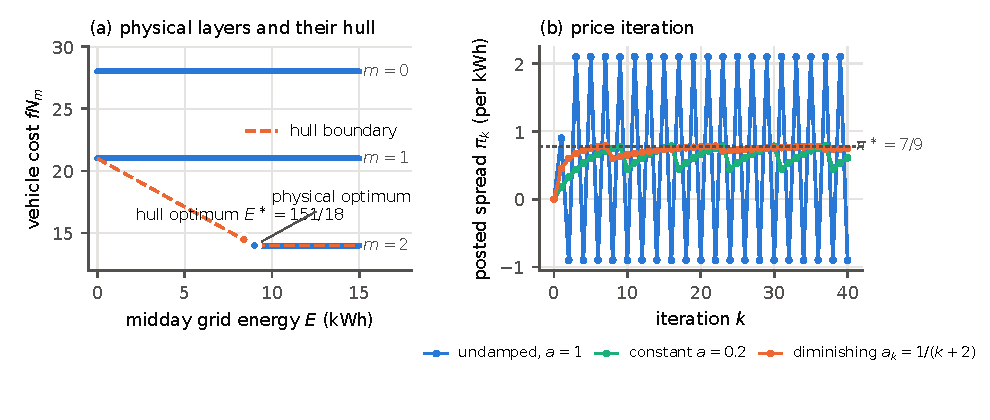
\includegraphics[width=\textwidth]{figures/anchor.pdf}
\caption{The worked example. (a)~Physical layers (solid) and the lower hull
boundary (dashed); the hull optimum lies strictly inside the sloping face, so
$\Delta>0$. (b)~Price iteration on the scalar spread $\pi=p_E-p_L$: undamped
prices enter a 2-cycle that alternates between loads $0$ and $15$. A constant
step $a=0.2$ keeps prices in a band around the convex-hull spread $\pi^*=7/9$
while loads alternate between $0$ and $9$. Diminishing steps converge to $\pi^*$.}
\label{fig:anchor}
\end{figure}

\section{Price formation on the exact class}\label{sec:prices}

We now use the exact description to answer the two questions from the
introduction for the lossless class \eqref{eq:lossless}. The same arguments apply
to the lossless bidirectional class, whose layers are intervals
$[t_m,U]$ with $t_m=\max\{S_0-H,\,S_0-N_mB,\,2r_m-K\}$ (\cref{app:projection}).

On the physical set, the terminal load is $S_0-E$. A posted price $p=(p_E,p_L)$
therefore charges $p_LS_0+\pi E$ with $\pi=p_E-p_L$, and the operator's response
depends only on the \emph{spread} $\pi$. Assume $\mathrm{Lo}<U$, and let $F$ be convex
and differentiable on a neighbourhood of the attainable loads. Let
let $g(E)=\partial_EF-\partial_LF$ at $(E,S_0-E)$. This is the marginal-cost spread
at early load $E$, and it equals $G'(E)$. Assume $g$ is continuous and strictly
increasing on $[\mathrm{Lo},U]$, let $E^*$ be the unique hull optimum, and let
$\pi^*=g(E^*)$, the \emph{convex-hull spread}. The response correspondence
$R(\pi)$ is the set of physical loads minimizing $fN_m+\pi E$. We use vertex
selections, which pick $R(\pi)$ among layer endpoints, as a linear-programming
solver would.

\paragraph{Anatomy of the gap.} A positive gap needs a sloping face that is
expensive enough to straddle, and its size is controlled by the face length.

\begin{proposition}[Gap conditions]\label{prop:anatomy}
Let $\eta_{\max}=\max_{m_0<m\le m_{\max}}\eta_m$ (zero if there is no sloping
face).
\begin{enumerate}[label=(\roman*),itemsep=1pt]
\item If $\Delta>0$, then $E^*$ lies strictly between consecutive breakpoints
$u<u'$ with $\pi^*=f/(u'-u)$. In particular $\max_{[\mathrm{Lo},U]}g\ge f/\eta_{\max}$:
no gap can occur when the vehicle cost exceeds $\eta_{\max}$ times the largest
marginal-cost spread.
\item If $g$ is $\kappa$-Lipschitz, then $\Delta\le\kappa(u'-u)^2/8\le\kappa\eta_{\max}^2/8$.
\end{enumerate}
\end{proposition}

Part (i) has a plain reading. Straddling a face means preferring a mixture of
``one more pair, $u'-u$ more kWh in the early window'' and ``one fewer pair''. That
is worthwhile only when the marginal spread prices the forced energy at the
vehicle cost it saves. Part (ii) says the gap, unlike the regret, is of second
order in the face length.

\paragraph{Price iteration.}
A natural way to find a supporting price is to post a price, observe the
fleet's response, and move the price toward the marginal cost of that response:
\begin{equation}\label{eq:iteration}
 \pi_{k+1}=(1-a_k)\pi_k+a_k\,g(E_k),\qquad E_k\in R(\pi_k),\quad a_k\in(0,1].
\end{equation}
Applied componentwise to $(p_E,p_L)$, the damped update
$p_{k+1}=(1-a_k)p_k+a_k\nabla F(e_k)$ induces exactly \eqref{eq:iteration} on the
spread. It is the natural damped fixed-point scheme for computing a price that
equals the marginal cost of the response it induces. A fixed point is a
spread with $\pi=g(E)$ for some selected $E\in R(\pi)$, that is, a supported
plan. The behaviour hinges on whether $E^*$ is a strict vertex of the hull
boundary or lies in the relative interior of a maximal face $[w,w']$, which may
be a sloping face (possibly containing further breakpoints) or the final flat one.

\begin{lemma}[Sign property]\label{lem:sign}
For every $\pi$ and every $E\in R(\pi)$, $(\pi-\pi^*)(g(E)-\pi^*)\le0$.
Consequently, for every step $a\in(0,1]$,
$|\pi_{k+1}-\pi^*|\le\max\{(1-a)|\pi_k-\pi^*|,\,aM\}$, where
$M=\max_{E\in[\mathrm{Lo},U]}|g(E)-\pi^*|$.
\end{lemma}

\begin{theorem}[Price iteration on the two-batch class]\label{thm:iteration}
Under the standing assumptions of this section:
\begin{enumerate}[label=(\alph*),itemsep=2pt]
\item \emph{Fixed points.} Some vertex selection has a fixed point if and only if
$E^*$ is a breakpoint or $E^*=U$. In particular there is no fixed point when $\Delta>0$, nor when $E^*$ lies
inside the flat face, although $\Delta=0$ in the latter case.
\item \emph{Undamped iteration} ($a_k\equiv1$, a deterministic selection). Every orbit is eventually
periodic with period one or two. If $E^*$ lies in the relative interior of a
maximal face $[w,w']$ and $\pi_0\neq\pi^*$, the period is two and the cycle's loads satisfy
$E_{\rm lo}\le w<w'\le E_{\rm hi}$.
\item \emph{Constant step} $a\in(0,1)$. Every orbit enters the interval
$|\pi-\pi^*|\le aM$ after finitely many steps and remains there. If $E^*$ is a strict
vertex in the interior of its normal cone, and $aM$ is smaller than the distance
from $\pi^*$ to the cone's boundary, then $\pi_k\to\pi^*$ geometrically and $E_k=E^*$
eventually. If $E^*$ lies in the relative interior of a maximal face $[w,w']$, the prices
converge for at most countably many initial prices, and for none if $E^*$ is not a
breakpoint. If moreover $aM$ is smaller than the distance from $\pi^*$ to the
far ends of the normal cones of $w$ and $w'$, then eventually every load lies in
$[w,w']$ and equals $w$ or $w'$ unless $\pi_k=\pi^*$ exactly; unless the orbit
reaches $\pi^*$ and the selection then picks $E^*$, both $w$ and $w'$ recur
infinitely often; and
$\pi_k\in[\pi^*-a\,d_-,\ \pi^*+a\,d_+]$ with $d_-=\pi^*-g(w)$ and $d_+=g(w')-\pi^*$.
\item \emph{Diminishing steps} ($a_k\to0$, $\sum_ka_k=\infty$). Then $\pi_k\to\pi^*$,
and the step-weighted averages of $g(E_k)$ converge to $\pi^*$. If $g$ is affine,
the step-weighted average load converges to $E^*$.
\end{enumerate}
\end{theorem}

\Cref{lem:sign} is the whole engine. It follows from monotonicity of the hull
boundary's subdifferential, and the proofs are in \cref{app:prices}.
\Cref{fig:anchor}b illustrates all three regimes on the worked example. The
step-size conditions in (c) matter. In the worked example with the steeper supply
$F(E,L)=16E+(E^2+L^2)/4$, the hull optimum is the supported vertex $E^*=9$, yet
undamped iteration from $\pi_0=3$ alternates between loads $0$ and $15$ forever,
while the step $a=1/10$ converges. Part (b) also assumes a selection that depends
only on the current price; history-dependent tie rules are outside its scope.

\paragraph{What the theorem says about cycling.} With small steps,
non-convergence of \eqref{eq:iteration} is caused by a \emph{degenerate tangency}: the optimal load
sits on a face of the frontier, where the linear response jumps between the
face's endpoints. That happens in two different situations. On a sloping face
the interior loads are not physical, so $\Delta>0$ and no posted price can
support any plan; side payments or schedule mixing over days are unavoidable.
On the flat face (the cheapest fleet has spare midday capacity) every interior
load is physical and supported at $\pi^*$, but a vertex-returning solver never
selects it. A tie-breaking rule or a quantity signal is then enough. Damping
cannot tell these apart, and neither can the presence of a cycle. The gap
$\Delta$, or equivalently whether $E^*$ is physical, is the right diagnostic.
The calibrated study in \cref{sec:study} shows that the second situation is the
common one.

\paragraph{What averaging buys.} Parts (c) and (d) give the hull a physical
meaning. Iterating with small steps and operating the visited schedules on
successive days implements, on average, the convex-hull plan. This is the
one-dimensional counterpart of ergodic primal recovery in dual subgradient
methods \citep{larsson1999ergodic,nedic2009approximate}, here with exact
identification of which two schedules alternate.

\section{Where the reduction stops}\label{sec:boundaries}

The reduction rests on one fact: at fixed cardinality, total energy and every
aggregate bound except the mandatory purchase are independent of the
matching. We now show which changes preserve that fact and which destroy it.

\paragraph{Common transition energy preserves it.} If every matched pair performs
the same compulsory task of energy $d\ge0$ during a noncharging interval
between the early window and the B batch, then total consumption is $S_0+md$, the
paired interval becomes $[a_i+b_j+d-B,a_i]$, and edges with $b_j+d>B$ are removed.
\Cref{thm:projection} holds with these substitutions
(\cref{app:boundaries}).

\paragraph{Edge-dependent transition energy breaks it.}
When the transition energy depends on the pair, total energy depends on the
matching, and a minimum-requirement matching no longer dominates.

\begin{proposition}[Support failure on a complete assignment graph]\label{prop:completegraph}
For every $k\ge1$ there is a charge-only two-batch instance with $2k$
services per batch, the complete assignment graph, pair-dependent compulsory
transition energies, and a fleet cap of $2k$, in which every perfect matching is
physically feasible and, for the strongly convex-in-$E$ supply
$F(E,L)=3E+L+(E-3)^2/(2K)$ and any $f\ge0$,
\[
 D=\CH+\frac{9}{2K}>\CH.
\]
\end{proposition}

The construction and proof are in \cref{app:boundaries}. Every assignment
alternative is admitted, so the gap is not an artifact of a sparse
compatibility graph or of infeasible pairings. The gap shrinks as $K$ grows; the
statement is an existence result, not a prevalence claim.

\paragraph{A third batch makes feasibility hard.}

\begin{proposition}[Three batches]\label{prop:threebatch}
With three successive batches of $n$ simultaneous services, complete zero-energy
compatibility between consecutive batches, no charging before the last batch,
fleet cap $n$ and an adequate terminal connector, deciding whether a feasible
fleet exists is strongly NP-complete.
\end{proposition}

The proof reduces from numerical three-dimensional matching
\citep[problem SP16]{garey1979} (\cref{app:boundaries}). Pairwise matching
therefore cannot describe longer duties, which is why the exact class stops at
two batches.

\paragraph{Positive setup time.} The construction in \cref{thm:projection} uses
arbitrarily many short neutral cycles and zero switching time. A positive setup
time per action breaks exactness: it can make a layer infeasible while
neighbouring layers stay feasible, and the number of buses needing early charge
then matters separately from $r_m$. A conservative inner approximation with
explicit slack conditions is possible; we leave a systematic treatment to future
work.

\paragraph{Beyond the class: one certified public timetable.}
To show that the obstruction is not an artifact of synchronized batches, we
certified a strictly positive gap on the 37-service Hildenbrand timetable from
the Sistig et al.\ dataset, using a single depot with its complete
deadhead matrix, varied service times, and one shared 360\,kW connector,
400\,kWh batteries and synthetic economics (vehicle cost 100,
$F(e)=\sum_{t=1}^{30}(0.2e_t+e_t^2/1800)$ over hourly intervals). A feasible
two-plan mixture bounds the hull from above. An exhaustive rational
branch-and-bound certificate, checked independently, bounds every physical fleet
from below:
\[
 \CH\le 441.142238<441.532912\le D\le 441.532913.
\]
By \cref{prop:support}, no physical schedule is supported at its own marginal
prices. The result holds under two separately certified energy models: the
dataset's stored consumption values on the declared movement graph, and an
exactly additive law covering arbitrary finite walks under triangle-inequality
premises. \Cref{app:public} summarizes the certificate and its scope. The gap
is about $0.09\%$ of $D$, consistent with the magnitudes in \cref{sec:study}.

\section{A calibrated study with public timetables}\label{sec:study}

The theory says when support can fail and how large the gap can be. We now ask
whether those conditions arise for real service energies.

\paragraph{Data and instance construction.}
The dataset of \citet{sistig2025dataset} (CC BY 4.0) contains timetables, stops
and directed deadhead matrices for German bus operators. For each of the 20
operators in the archive we take the weekday day type with the most service
trips. Trips departing in the morning peak $[05{:}30,09{:}30)$ form the A batch
and trips departing in the afternoon peak $[14{:}30,18{:}30)$ form the B batch.
Within each batch we chain trips into the minimum number of vehicle runs
(maximum bipartite matching on the reachability graph). Each run's energy uses
the source study's vehicle parameters: 1.2\,kWh/km in service, 0.96\,kWh/km
deadheading, and 16\,kWh/h of auxiliary load away from the depot, including
pull-out and pull-in to the nearest depot \citep{sistig2025electrification}. We
drop 108 trip records whose implied speed exceeds 90\,km/h as data errors, and the two
operators with fewer than five runs per batch. This leaves 18 operators with
6--413 morning runs and 6--298 afternoon runs. The 3913 run energies have
median 154\,kWh and interdecile range 110--204\,kWh. The resulting instances keep the real heterogeneity of peak-run
energies and nothing else: off-peak service, crews and multi-depot structure are
not modeled.

\paragraph{Economics.} We treat economics as a sensitivity grid rather than a
calibration. The daily vehicle cost is $f=150$\,EUR in the sweeps; critical
spreads scale linearly in $f$. The supply cost in each window is quadratic,
$\bar p_wE+\beta E^2/2$, so the marginal-cost spread is
$g(E)=s_0+\beta(2E-S_0)$, which is Lipschitz with $\kappa=2\beta$. The zero-load
spread $s_0=\bar p_E-\bar p_L$ ranges over 37 values from $-0.2$ to
$1.6$\,EUR/kWh. The price impact is $\beta=\rho\,\bar p/S_0$ with $\bar p=0.15$\,EUR/kWh
and $\rho\in\{0.5,1,2,4\}$: drawing the fleet's whole daily energy in one window
would raise that window's marginal cost by $\rho\bar p$. We report costs relative
to the total daily cost, vehicles plus energy, with the overnight zero-load price
set to $\bar p$. The midday budget $K$ is either ample ($K=P$) or half that, and
the overnight budget is ample. The model has no in-service charging, so a run
needing more than the usable battery $B$ cannot be served. We exclude such
operator--battery combinations rather than trimming their runs (57 runs exceed
250\,kWh, 13 exceed 300\,kWh, 8 exceed 350\,kWh, none exceed 400\,kWh).

\paragraph{Result 1: with today's batteries the obstruction is mostly impossible.}
\Cref{prop:anatomy}(i) turns the data into a necessary condition: a gap requires
a marginal spread of at least $f/\eta_{\max}$, which depends only on run energies
and battery size. \Cref{fig:critical} shows it per operator. With $B=400$\,kWh,
15 of 18 operators have $r_m=0$ for every $m$: every pairing of a morning and an
afternoon run needs no midday charging. The frontier is then flat, and support
cannot fail at any price. For the remaining three the critical spread is
0.53\,EUR/kWh or more, and above 35\,EUR/kWh for two of them. Smaller batteries
make forced charging real. At $B=350$\,kWh, 5 of 17 eligible operators admit a gap,
from 0.81\,EUR/kWh (median 1.40). At $B=300$\,kWh, 8 of 14 do, from 0.91\,EUR/kWh
(median 1.27). At $B=250$\,kWh, all 9 eligible operators do, from 0.72\,EUR/kWh
(median 1.70). These thresholds are several times the 0.15\,EUR/kWh reference
energy price. Support failure therefore needs capacity or scarcity pricing, or a
much cheaper vehicle, together with a battery sized close to the paired energy.

\begin{figure}[t]
\centering
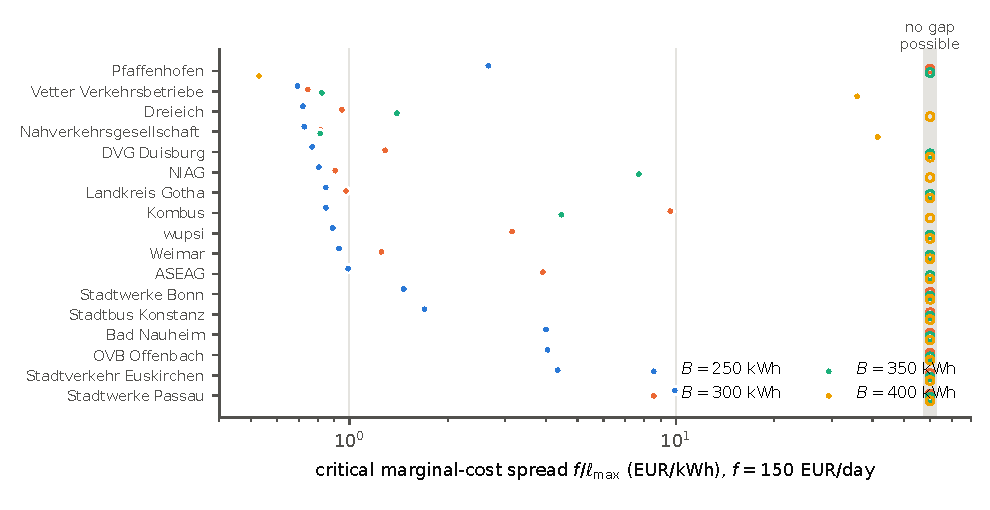
\includegraphics[width=\textwidth]{figures/critical.pdf}
\caption{Critical marginal-cost spread $f/\eta_{\max}$ below which no support
gap can occur (\cref{prop:anatomy}), for a vehicle cost of 150\,EUR/day, per
operator and usable battery size $B$. Hollow markers: $r_m=0$ for all $m$, so no
gap is possible at any price. Crosses: some peak run needs more than $B$, so the
combination is outside the model.}
\label{fig:critical}
\end{figure}

\paragraph{Result 2: gaps are rare and small; regret is not.}
At $B=400$\,kWh the grid has $18\times37\times4=2664$ scenarios. Only 7 have
$\Delta>0$, all with $s_0>0.3$\,EUR/kWh, and the largest gap is 0.023\% of total
daily cost. At $B=300$\,kWh (14 eligible operators, 2072 scenarios) there are 6,
with gaps up to 0.054\%. In gap scenarios, the planner optimum's regret at its own
marginal prices is a median 8.5 times the gap at $B=400$ (4.2 at $B=300$). The
operator's incentive to deviate is several times the welfare at stake, as in the
worked example. Halving the midday budget leaves these gap counts unchanged.

\paragraph{Result 3: cycling is common and mostly unrelated to the gap.}
Undamped iteration, started from the spread at the smallest attainable early
load, cycles in 397 of the 2664 scenarios at $B=400$\,kWh (15\%). Of these, 390 have
$\Delta=0$ (\cref{fig:sweep}). Classifying the hull optimum explains them: it lies
inside the flat face in 384 cycling scenarios, inside a sloping face in 7 (exactly
the gap scenarios) and at a vertex in 6, where the undamped step is too large
for part (c) of \cref{thm:iteration}. Every scenario with a face optimum cycles.
The flat-face cases concentrate at small spreads: the cheapest fleet has spare
midday capacity, and the vertex response jumps between the two ends of its
interval. With half the midday budget, 189 scenarios (7\%) cycle, 182 of them
without a gap. At $B=300$\,kWh the pattern is the same: 307 of 2072 cycle and 301
of these have no gap. A study that counted price cycles as evidence of
assignment nonconvexity would overstate it by a factor of about fifty here.

\begin{figure}[t]
\centering
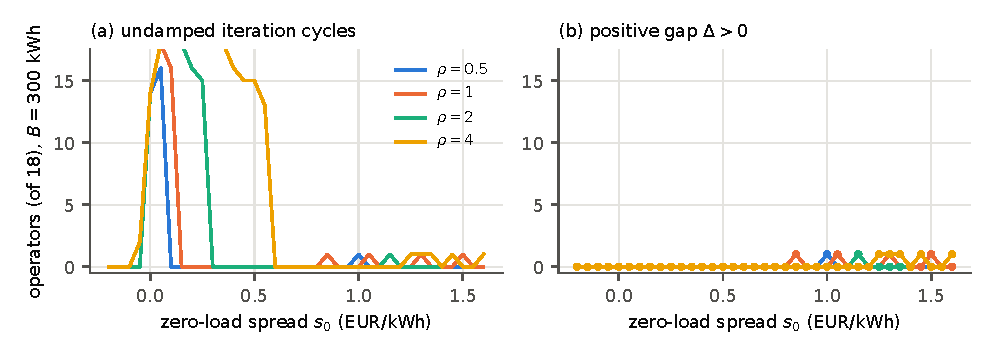
\includegraphics[width=\textwidth]{figures/sweep.pdf}
\caption{Number of operators (of 18; $B=400$\,kWh, $f=150$\,EUR/day, ample midday
budget) whose undamped price iteration cycles (a) and whose planning problem has a
positive gap (b), as functions of the zero-load spread $s_0$ and the price impact
$\rho$. Cycling concentrates at small spreads with no gap.}
\label{fig:sweep}
\end{figure}

\section{Discussion}\label{sec:discussion}

\paragraph{For tariff design.} The exact class isolates the economic content of
assignment nonconvexity. A depot facing a marginal-cost tariff will under- or
over-charge at midday only when the spread prices forced charging at the
vehicle cost it saves. That requires battery capacity close to the paired energy
of peak runs, together with a spread near $f/\eta$. When it happens, the
welfare loss is second order, at most $\kappa\eta^2/8$, but the operator's bill
regret is first order. At the convex-hull price an uplift of at most $\Delta$
supports the planner optimum (\cref{sec:model}). That is far cheaper than
compensating the regret at the operator's own marginal prices, and it works where
re-pricing until convergence does not.

\paragraph{How much the price-maker concern matters.} The calibrated study gives
a sober answer for peak operations. With current battery sizes, most operators'
peak runs pair freely, and the assignment nonconvexity is invisible to any
price. Where it is visible, it needs spreads several times the reference
energy price, and the welfare at stake is a few hundredths of a percent of daily cost.
The operator's incentive to deviate, however, is several times larger. The
binding consideration for tariff design is therefore the incentive problem, not
the efficiency loss. Battery downsizing, demand charges and scarcity pricing all
push depots toward the regime where the obstruction appears, so the threshold
$f/\eta_{\max}$ is the quantity to monitor.

\paragraph{For price-coordination algorithms.} \Cref{thm:iteration} separates
two causes of non-convergence. Degenerate flat-face responses can be removed by
selection rules, such as choosing the response closest to the previous load or
announcing a target quantity. Sloping-face gaps cannot be removed by any price.
Constant damping only narrows the band, and an overly large step can make prices
cycle even around a supported vertex. Diminishing steps with averaging recover
the hull plan. Iterative tariff negotiation between a depot and a supplier
should therefore report the gap, or a certificate that $E^*$ is physical,
rather than a cycle count.

\paragraph{Limitations.} The exact theorem assumes two synchronized batches,
common availability and efficiencies, zero-time transitions, ideal switching
and period-aggregate settlement. \Cref{sec:boundaries} shows that
edge-dependent transitions and a third batch are genuine boundaries, and that
setup time requires separate treatment. The calibrated study uses real service
energies but stylized peak runs and illustrative economics. It is not an
estimate of savings for any operator. The 37-service certificate establishes
existence beyond the class for one timetable with synthetic economics.

\paragraph{Open directions.} Three extensions would most increase reach: a
characterization for staggered charging windows, where serialization is no
longer automatic; an approximate reduction with setup time and its error
bound; and an analysis of the strategic operator who anticipates the
price change, for which the exact projection is the natural strategy space.

\bibliographystyle{plainnat}
\bibliography{references}

\appendix
\section{Proofs for Section~\ref{sec:projection}}\label{app:projection}

\subsection{Proof of Theorem~\ref{thm:projection}}
Fix one allowed matching $M$ with $|M|=m$, fleet $N=N_m$, requirement
$R=\sum_{(i,j)\in M}(a_i+b_j-B)_+$ and $T=S_0-NB$. Let $x_v$ be a bus's net early
battery gain. A paired bus serving $A_i$ and $B_j$ holds $B-a_i$ after its
morning service; it cannot exceed capacity, so $x_v\le a_i$, and it must hold at
least $b_j$ before the afternoon service, so $x_v\ge a_i+b_j-B$. An A-only bus
has $x_v\in[a_i-B,a_i]$, and a B-only bus, full before the early window, has
$x_v\in[b_j-B,0]$. These boxes are nonempty because $a_i,b_j\le B$. Their lower
endpoints sum to $T$, their positive lower endpoints to $R$, and their upper
endpoints to $P$; every upper endpoint is nonnegative.

\emph{Necessity.} Whatever the order of actions, $x_v=\alpha C_v-X_v/\delta$ for
the bus's early purchases $C_v$ and exports $X_v$, so the total $Q$ lies in
$[T,P]$. A positive lower endpoint needs at least its value divided by $\alpha$
in purchases, hence $C\ge R/\alpha$. Exports are nonnegative, the shared
connector carries gross energy $C+X\le K$, and full terminal replenishment
needs the terminal purchase $L=(S_0-Q)/\alpha\le H$. Terminal purchases are
nonnegative because $Q\le P<S_0$.

\emph{Sufficiency.} Fix totals $(C,X)$ satisfying these inequalities with $R$ in
place of $r_m$. For any $Q\in[T,P]$ the boxes admit gains whose positive parts
sum to $A=\max\{R,Q\}$. If $Q\ge R$, start from the positive lower endpoints and
zero elsewhere, and distribute $Q-R$ through the remaining headroom. If $Q<R$,
keep the mandatory positive gains and distribute the negative total $Q-R$
through the negative lower intervals, whose combined lower endpoint is $T-R$.
One-direction exchanges then realize $C_0=A/\alpha$ and $X_0=\delta(A-Q)$. Since
$X\ge0$ implies $\alpha C\ge Q$, and $\alpha C\ge R$, the residual $z=C-C_0$ is
nonnegative and $X-X_0=\alpha\delta z$.

Realize these residuals by battery-neutral cycles on one bus before its
one-direction exchange. At early state of charge $s\in[0,B]$, use
charge-then-discharge cycles of depth at most $B-s$ if $s\le B/2$, and
discharge-then-charge cycles of depth at most $s$ otherwise. The permitted depth
is at least $B/2>0$. Split the residual battery throughput $\alpha z$ into
finitely many such chunks. Each returns to $s$, stays in $[0,B]$, and uses grid
purchases depth$/\alpha$ and exports $\delta\cdot$depth, so together they
realize exactly $(z,\alpha\delta z)$. Execute the cycles and then all
one-direction exchanges serially: their gross energy is $C+X\le K$, so they fit
the common early window at the connector's power. The endpoint boxes guarantee
the afternoon service, and nonnegative service draw preserves every
intermediate state-of-charge bound. Refill serially at the terminal connector
using total $L\le H$. If $K=0$ all early actions vanish; if $H=0$, then $P<S_0$
makes every polygon empty, consistent with infeasibility.

\emph{Replacement.} At fixed $m$, the quantities $S_0,P,N_m,T$ and the fleet cost
do not depend on the matching; only $R$ does, and only through $C\ge R/\alpha$.
Hence the polygon of a matching attaining $r_m$ contains the polygon of every
other matching of size $m$, and every point of it has just been realized.
The union over matchings of size $m$ therefore equals the polygon $W_m$, and the
union over $m$ gives $\mathcal P$. Each $W_m$ is defined by five half-planes, so
it has at most five vertices, and $\conv\mathcal P$ is the convex hull of their
images. With exports prohibited, the construction above uses no exports when
$X=0$: then $\alpha C=Q\ge R$, so $A=Q$, $X_0=0$ and $z=0$. \qed

\paragraph{Idle buses.} Identical paid idle buses under the total fleet cap
$n_A+n_B$ do not change $\mathcal P$. An idle bus has the box $[-B,0]$. A plan
with $m$ pairs and $q$ idle buses has $q\le m$ by the cap; deleting $q$ pairs
and serving their services separately preserves $N,S_0,P,T$ and the fleet cost
while lowering $R$, and reproduces the same $(C,X)$.

\subsection{The lossless cases}
\emph{Charge-only.} With $\alpha=\delta=1$ and $X=0$, $W_m$ becomes
$\{C:\ C\ge r_m,\ C\le K,\ S_0-N_mB\le C\le P,\ C\ge S_0-H\}$. Since
$S_0-N_mB$ is the sum of all lower endpoints and $r_m$ the sum of their positive
parts, $S_0-N_mB\le r_m$, and the layer is $\{E:\max\{\mathrm{Lo},r_m\}\le E\le U\}$ with
$L=S_0-E$, which is \eqref{eq:lossless}. Feasibility is $\mathrm{Lo}\le U$ because the empty
matching has $r_0=0$.

\emph{Bidirectional.} With $\alpha=\delta=1$ and exports allowed, $E=C-X$ and
$L=S_0-E$. A point $E$ is attainable in layer $m$ if and only if
$\max\{S_0-N_mB,S_0-H\}\le E\le P$ and some $C\ge\max\{r_m,E\}$ satisfies
$2C-E\le K$, that is, $E\le K$ and $E\ge2r_m-K$. The layer is therefore
$[t_m,U]$ with $t_m=\max\{S_0-H,\,S_0-N_mB,\,2r_m-K\}$ and $U=\min\{P,K\}$.

\subsection{Monotonicity, convexity and the frontier}
Deleting an edge from a minimum matching of size $m$ shows $r_{m-1}\le r_m$.
For discrete convexity, consider the unit-capacity source--A--B--sink network on
the allowed edges with costs $(a_i+b_j-B)_+$. Its minimum-cost flow LP is
integral at integer flow values $m=0,\dots,\nu$, and its value is convex in the
required flow, so $2r_m\le r_{m-1}+r_{m+1}$. This uses bipartiteness, not
completeness of $\Gamma$.

All thresholds at or below $\mathrm{Lo}$ are dominated in cost by $m_0$. The first retained
increment is $r_{m_0+1}-\mathrm{Lo}\le r_{m_0+1}-r_{m_0}$, and later increments are the
original nondecreasing matching increments, all positive after $m_0$. The slopes
$-f/\delta_m$ are therefore nondecreasing, followed by the flat segment.
Endpoints are physical, interpolants are hull mixtures, and every physical
branch lies on or above this convex graph, so the graph is exactly the lower
hull boundary. Consecutive breakpoints differ by one cardinality.

\subsection{Proof of Corollary~\ref{cor:support}}
The convex frontier plus strictly convex continuous $G$ has a unique minimizer
$E^*$. At $\mathrm{Lo}$, at a breakpoint or on the flat segment, a physical plan attains
the frontier, so $D=\CH$. Strictly between consecutive breakpoints the frontier's
operating cost is strictly below that of every physical branch because $f>0$, so no
physical plan attains the hull optimum; compactness of the finite union of
physical segments then gives $D>\CH$.

\subsection{Sorted matching for the complete graph}
Replacing a selected service by an unused smaller draw while keeping its partner
cannot increase the nondecreasing edge cost, so some optimal size-$m$ matching
uses the $m$ smallest draws in each batch. With $h(t)=(t-B)_+$ and $a\le a'$,
$b\le b'$, convexity gives $h(a+b)+h(a'+b')\ge h(a+b')+h(a'+b)$. Swapping any
two partners ordered in the same direction therefore cannot raise the cost, and
repeated exchanges yield opposite order. For a non-complete graph this shortcut
fails: with A draws $(5,15)$, B draws $(14,15)$ and $B=20$, allowing only the
index-matched edges gives $r_2=10$ instead of $9$.

\subsection{The worked example}
The requirement matrix is $\bigl(\begin{smallmatrix}0&0\\9&10\end{smallmatrix}\bigr)$,
so $r_0=r_1=0$, $r_2=9$, $S_0=49$, $\mathrm{Lo}=0$ and $U=15$. With
$G(E)=2401/20-9E/10+E^2/10$, the physical minima of layers $m=0,1$ are at $E=9/2$,
with values $5841/40$ and $5561/40$; layer $m=2$ is minimized at its endpoint
$E=9$ with value $2681/20$. On the sloping hull face the objective is
$2821/20-151E/90+E^2/10$, minimized at $E^*=151/18$ with value $434201/3240$, so
$\Delta=121/3240$. The hull point mixes the three-bus plan at $E=0$ and the
two-bus plan at $E=9$ with weights $11/162$ and $151/162$. At the physical
optimum's marginal prices $(49/10,4)$ each layer's bill is minimized at its lowest
endpoint; bill plus vehicle cost is $224$, $217$ and $2181/10$, so the regret is
$11/10$. Both mixed plans have explicit serial witnesses: at $E=0$ pair the 5-draw
A with the 14-draw B and refill $19,15,15$ on the terminal connector; at $E=9$ the
15-draw A bus charges $9$ at midday in the crossed pairing and both buses refill
$20$.

\section{Proof of Proposition~\ref{prop:support}}\label{app:support}
For any hull point $(e,c)$, linear minimization gives $c+p^\top e\ge V(p)$. If
$p\in\partial F(e(x))$, then $F(e)\ge F(e(x))+p^\top(e-e(x))$. Adding and
minimizing over the hull gives $\CH\ge V(p)+F(e(x))-p^\top e(x)=c(x)+F(e(x))-r(x;p)$,
which is the regret bound; if $r(x;p)=0$, then $D=\CH$.

Conversely let $D=\CH$. Compactness gives a physical minimizer $x$. The
relative-interior condition gives strong Fenchel duality with an attained
maximizer, $\CH=V(p^*)-F^*(p^*)$. Then
\[
 \underbrace{c(x)+(p^*)^\top e(x)-V(p^*)}_{\ge0}
 +\underbrace{F(e(x))-(p^*)^\top e(x)+F^*(p^*)}_{\ge0}=D-\CH=0,
\]
so both terms vanish: Fenchel equality gives $p^*\in\partial F(e(x))$, and the
first term gives $r(x;p^*)=0$. \qed

\section{Proofs for Section~\ref{sec:prices}}\label{app:prices}

Throughout, $\bar c$ is the lower hull boundary on $[\mathrm{Lo},U]$, extended by
$+\infty$ outside, and $H(\pi)=\arg\min_E\{\bar c(E)+\pi E\}$ is the hull response.
The finite candidate set $\mathcal V$ consists of all layer endpoints $(\ell_m,fN_m)$
and $(U,fN_m)$. Since a linear function attains its minimum over $\conv\mathcal P$
at a point of $\mathcal V$, every $E\in R(\pi)$ satisfies $\bar c(E)=fN_m$ for its
layer and $E\in H(\pi)$. The layer endpoints that lie on $\bar c$ are exactly the
breakpoints $\mathrm{Lo}$, $r_m$ ($m_0<m\le m_{\max}$) and $U$. The hull optimum satisfies
$-\pi^*\in\partial\bar c(E^*)$ because $G$ is differentiable.

\subsection{Proof of Proposition~\ref{prop:anatomy}}
(i) By \cref{cor:support}, $\Delta>0$ places $E^*$ strictly between consecutive
breakpoints $u<u'$, where $\bar c$ is affine with slope $-f/(u'-u)$ because
consecutive breakpoints differ by one cardinality. Optimality at an interior point
gives $g(E^*)=f/(u'-u)\ge f/\delta_{\max}$, and $\max g\ge g(E^*)$.

(ii) On $[u,u']$ let $\phi=\bar c+G$. Then $\phi'(E)=-f/(u'-u)+g(E)$ is
$\kappa$-Lipschitz and vanishes at $E^*$, so $\phi(E)-\phi(E^*)\le\kappa(E-E^*)^2/2$.
Both $u$ and $u'$ are physical with cost $\bar c$, so
$D\le\min\{\phi(u),\phi(u')\}$ while $\CH=\phi(E^*)$. One of $u,u'$ is within
$(u'-u)/2$ of $E^*$, which gives $\Delta\le\kappa(u'-u)^2/8$. \qed

\subsection{Proof of Lemma~\ref{lem:sign}}
Let $E\in R(\pi)\subseteq H(\pi)$, so $-\pi\in\partial\bar c(E)$, and recall
$-\pi^*\in\partial\bar c(E^*)$. Monotonicity of the subdifferential of the convex
function $\bar c$ gives $(-\pi+\pi^*)(E-E^*)\ge0$, that is, $(\pi-\pi^*)(E-E^*)\le0$.
Since $g$ is increasing and $g(E^*)=\pi^*$, $(\pi-\pi^*)(g(E)-\pi^*)\le0$. For the
second claim write
$\pi_{k+1}-\pi^*=(1-a)(\pi_k-\pi^*)+a(g(E_k)-\pi^*)$. The two terms have
opposite (weak) signs, and for real $x,y$ with $xy\le0$, $|x+y|\le\max\{|x|,|y|\}$.
Since $E_k\in[\mathrm{Lo},U]$, $|g(E_k)-\pi^*|\le M$. \qed

\subsection{Proof of Theorem~\ref{thm:iteration}}
We use three facts. (F1) The same monotonicity argument shows that $\pi<\pi'$,
$E\in H(\pi)$ and $E'\in H(\pi')$ imply $E\ge E'$. (F2) If $E^*$ lies in the relative
interior of a maximal face $[w,w']$, then $\partial\bar c(E^*)=\{-\pi^*\}$, the face
has slope $-\pi^*$, $[w,w']\subseteq H(\pi^*)$, and $E^*\in H(\pi)$ only for
$\pi=\pi^*$. By (F1), $H(\pi)\subseteq[\mathrm{Lo},w]$ for $\pi>\pi^*$ and
$H(\pi)\subseteq[w',U]$ for $\pi<\pi^*$. (F3) A fixed point $\hat\pi=g(\hat E)$ with
$\hat E\in R(\hat\pi)$ has $-g(\hat E)\in\partial\bar c(\hat E)$, so $\hat E$
minimizes the convex function $\bar c+G$; by uniqueness $\hat E=E^*$ and
$\hat\pi=\pi^*$.

\emph{(a)} By (F3), a fixed point requires $E^*\in R(\pi^*)$ to be a selectable
layer endpoint on $\bar c$, that is, a breakpoint. Conversely, if $E^*$ is a
breakpoint then $E^*\in H(\pi^*)$ is a candidate attaining the minimum, so
$E^*\in R(\pi^*)$ and a selection choosing it makes $\pi^*$ a fixed point. If
$\Delta>0$, $E^*$ is not physical and hence not a breakpoint; if $E^*$ lies inside
the flat face $(\ell_{m_{\max}},U)$ it is physical but not a breakpoint.

\emph{(b)} Let $\sigma$ be the selection, a function of $\pi$ with values in
$R(\pi)$; by (F1) it is nonincreasing, so $h=g\circ\sigma$ is nonincreasing and
$h\circ h$ is nondecreasing. For $k\ge1$, $\pi_k$ lies in the finite set
$g(\{E:(E,c)\in\mathcal V\})$. The odd and even subsequences are orbits of the
nondecreasing map $h\circ h$, hence monotone, hence eventually constant in a finite
set. Thus $\pi_{k+2}=\pi_k$ eventually. In the face case with $\pi_0\neq\pi^*$, we
show by induction that $\pi_k\ne\pi^*$: if $\pi_k\neq\pi^*$ then by (F2)
$E_k\ne E^*$, so $\pi_{k+1}=g(E_k)\ne\pi^*$. By (F3) there is then no fixed
point along the orbit, and the period is two. If $\pi_a>\pi^*$ is one state of the
cycle, (F2) gives $E_a\le w<E^*$, hence $\pi_b=g(E_a)<\pi^*$ and $E_b\ge w'$.

\emph{(c)} By \cref{lem:sign}, $d_k=|\pi_k-\pi^*|$ satisfies
$d_{k+1}\le\max\{(1-a)d_k,aM\}$, so $d_k\le\max\{(1-a)^kd_0,aM\}$ and the
interval $d\le aM$ is reached in finitely many steps and is invariant.

\emph{Vertex case.} If $\pi^*$ is interior to the normal cone
$\{\pi:E^*\in H(\pi)\}$ and $aM$ is less than its distance to the cone's boundary,
then inside the invariant interval $H(\pi)=\{E^*\}$, so $E_k=E^*$ and
$\pi_{k+1}-\pi^*=(1-a)(\pi_k-\pi^*)$.

\emph{Face case: non-convergence.} Suppose $\pi_k\to\bar\pi$. Then
$a(g(E_k)-\pi_k)=\pi_{k+1}-\pi_k\to0$, so $g(E_k)\to\bar\pi$. Since $E_k$ ranges over a
finite set and $g$ is injective, $E_k=\bar E$ for all large $k$, with
$\bar\pi=g(\bar E)$. The set $\{\pi:\bar E\in R(\pi)\}$ is closed, being defined by
finitely many weak linear inequalities, so $\bar E\in R(\bar\pi)$, and (F3) gives
$\bar E=E^*$ and $\bar\pi=\pi^*$. If $E^*$ is not a breakpoint it is never selected,
which is a contradiction. If it is a breakpoint, $E^*\in R(\pi_k)$ forces
$\pi_k=\pi^*$ by (F2), so the orbit hits $\pi^*$ exactly. For a fixed sequence of
selected loads, $\pi_k$ is affine in $\pi_0$ with slope $(1-a)^k\neq0$, so each
finite selection sequence admits at most one such $\pi_0$, and there are countably
many sequences.

\emph{Face case: trapping.} Write $[\pi^*,\sigma]$ for the normal cone of $w$ and
$[\sigma',\pi^*]$ for that of $w'$ (with $\sigma=+\infty$ if $w=\mathrm{Lo}$ and
$\sigma'=-\infty$ if $w'=U$), and assume $aM<\min\{\sigma-\pi^*,\pi^*-\sigma'\}$.
Inside the invariant interval, $\pi>\pi^*$ forces $E=w$ and $\pi<\pi^*$ forces
$E=w'$; at $\pi=\pi^*$ the selection is a breakpoint in $[w,w']$. With
$d_-=\pi^*-g(w)>0$ and $d_+=g(w')-\pi^*>0$, an update from $\pi>\pi^*$ gives
$\pi'=(1-a)\pi+ag(w)\in[\pi^*-ad_-,\pi)$, and symmetrically from below; from
$\pi^*$ the update stays in $[\pi^*-ad_-,\pi^*+ad_+]$. This band is therefore
invariant. Above $\pi^*$, prices contract geometrically toward $g(w)<\pi^*$ and cross
$\pi^*$ in finitely many steps; below, they contract toward $g(w')>\pi^*$. Hence
the band is entered and both $w$ and $w'$ recur infinitely often.

\emph{(d)} With $d_{k+1}\le\max\{(1-a_k)d_k,a_kM\}$, fix $\varepsilon>0$ and $K$ with
$a_kM<\varepsilon$ for $k\ge K$. After $K$, the interval $d\le\varepsilon$ is invariant,
and outside it $d$ contracts by the factors $1-a_k$, whose product diverges to
zero because $\sum a_k=\infty$. Thus $\limsup d_k\le\varepsilon$ for every
$\varepsilon$. Summing the update gives $\sum_{k<K}a_k(g(E_k)-\pi_k)=\pi_K-\pi_0$,
which is bounded; dividing by $A_K=\sum_{k<K}a_k\to\infty$ and using
$\pi_k\to\pi^*$ (Stolz--Ces\`aro) gives $\sum_{k<K}a_kg(E_k)/A_K\to\pi^*$. If $g$
is affine, this average equals $g\bigl(\sum_{k<K}a_kE_k/A_K\bigr)$, and invertibility
of $g$ gives the load statement. \qed

\paragraph{Numerical verification.} The repository contains an exact
rational-arithmetic implementation of the projection, hull, gap and iteration
(\texttt{code/twobatch.py}) and randomized checks of every statement in this
section on several thousand instances: the period and bracketing claims in (b);
the absence of fixed points; trapping, band and recurrence in (c) at half the
stated step threshold; convergence in (d); and both parts of
\cref{prop:anatomy}. Instances are drawn so that the hull optimum falls on
sloping faces, flat faces and vertices.

\section{Proofs for Section~\ref{sec:boundaries}}\label{app:boundaries}

\subsection{Common transition energy}
Suppose every matched pair performs a compulsory task of energy $d\ge0$, with
nonnegative draw, during a noncharging interval after the early window and
before the B batch. A paired bus then needs $x_v\ge a_i+b_j+d-B$ to finish its
afternoon service, cannot exceed $x_v\le a_i$, and needs terminal refill
$a_i+b_j+d-x_v$. The box is nonempty exactly when $b_j+d\le B$, so edges
violating this are removed. Lower endpoints sum to $S_m-N_mB$ with
$S_m=S_0+md$, positive lower endpoints to the matching's requirement with $d$
included, and the upper endpoints still to $P$. Because $S_m$ depends only on $m$,
the proof of \cref{thm:projection} applies verbatim with $S_0$ replaced by $S_m$.

\subsection{Proof of Proposition~\ref{prop:completegraph}}
\emph{A disjoint-block construction.} Let $w_i=2^i$ for $i=0,\dots,k-1$,
$W=\sum_iw_i$, $B=20\max_iw_i$. Block $i$ has two A and two B services with draws
$(B/2+3w_i,\,w_i)$ in each batch. Use windows A $[0,1]$, early charging $[1,2]$,
noncharging transition tasks $[2,3]$, B $[3,4]$ and terminal charging $[4,5]$; one
early connector of budget $K=kB/2+4W$ and one terminal connector. Within a block,
the identity edges carry transition energy $0$ and the cross edges $6w_i$. The fleet
cap is $2k$, so exactly $2k$ buses are used and every bus serves one service from
each batch. Identity requires early purchase $6w_i$ and consumes $B+8w_i$; cross
requires none and consumes $B+20w_i$. For a set $I$ of identity blocks, with
$R=6\sum_{i\in I}w_i$ and $S_{\max}=kB+20W$, total consumption is $S_{\max}-2R$, the
per-bus early intervals sum to $[R,K]$, and the complete branch is
$\{(E,\,S_{\max}-2R-E,\,2kf):R\le E\le K\}$, each point realized by serial charging.

\emph{Complete graph.} Now admit every A--B edge. Keep the within-block transition
energies, and on each edge between different blocks set $d_{ij}=B-b_j$; raise the
terminal budget to $H=2kB$. For any edge put $e_{ij}=a_i+b_j+d_{ij}$ and
$r_{ij}=(e_{ij}-B)_+$. Its early purchase interval is $[r_{ij},a_i]$ whenever
$b_j+d_{ij}\le B$, which holds for within-block edges because $B\ge20\max w_i$ and
with equality between blocks. In the latter case $e_{ij}=a_i+B$ and $r_{ij}=a_i$: the
bus refills completely at midday. For a perfect matching $M$ these intervals sum
to $[R_M,K]$ with $R_M=\sum_Mr_{ij}$, total consumption is $S_M=\sum_Me_{ij}$, and the
branch is $L=S_M-E$, $R_M\le E\le K$. Each terminal purchase is at most
$e_{ij}-r_{ij}\le B$, so $H=2kB$ accommodates it; $E=K$ is feasible for every
perfect matching.

Give each high service (draw $B/2+3w_i$) in block $i$ the potential $B/2+9w_i$ and
each low service the potential $w_i$, as row potentials $u_i$ and column potentials
$v_j$; their total is $S_{\max}$. Every within-block edge satisfies
$e_{ij}+2r_{ij}=u_i+v_j$. A between-block edge has $e_{ij}+2r_{ij}=B+3a_i$, with slack
over $u_i+v_j$ equal to $3B/2-9w_j$, $2B-w_j$, $B/2+2w_i-9w_j$ or $B+2w_i-w_j$ for the
four high/low combinations. Each is at least $\gamma=w_{\max}+2w_{\min}\ge3$, the
low-to-high case being limiting because $B/2\ge10w_{\max}$. Summing this
assignment-potential certificate over $M$ gives $S_M+2R_M\ge S_{\max}$, with surplus at
least $\gamma$ if any between-block edge is used. Hence every physical point, and
every mixture, satisfies $3E+L=S_M+2E\ge S_M+2R_M\ge S_{\max}$.

With $F(E,L)=3E+L+(E-3)^2/(2K)$, total cost is at least $2kf+S_{\max}$. The equal
mixture of the within-block corners $R=0$ and $R=6$ attains it at load
$(3,S_{\max}-9)$, so $\CH=S_{\max}+2kf$. On a within-block branch the cost is
$2kf+S_{\max}+2(E-R)+(E-3)^2/(2K)$, increasing in $E$ (derivative at least
$2-3/K>0$ since $K\ge14$), hence minimized at $E=R$; the values $R=6t$ nearest to 3
are $0$ and $6$, giving excess $9/(2K)$. Every between-block schedule has excess at
least $\gamma\ge3>9/(2K)$. Therefore $D=\CH+9/(2K)$. \qed

\subsection{Proof of Proposition~\ref{prop:threebatch}}
Reduce from numerical three-dimensional matching, strongly NP-complete
\citep[SP16]{garey1979}: three multisets of $n$ positive integers must be
partitioned into triples, one from each, each summing to $B$. We may assume total
$nB$ and every number at most $B$, mapping violations to a fixed NO instance. Make
the multisets services in $[0,1)$, $[1,2)$ and $[2,3)$ with those numbers as
battery draws, with charging unavailable before time 3. Overlap and the fleet cap
force exactly $n$ buses, each serving one service per batch; a duty $(a,b,c)$ is
feasible exactly when $a+b+c\le B$, and the total $nB$ forces equality. Conversely, a
matching yields duties ending empty, which refill serially for $B$ time units each
during $[3,3+nB]$. The construction is polynomial and preserves strong hardness;
membership in NP is immediate. \qed

\section{The certified public timetable}\label{app:public}
The case uses the Hildenbrand timetable of \citet{sistig2025dataset}: 37 mandatory
services, the complete directed $5\times5$ deadhead matrix, and depot 15 as the sole
charging and parking location. Service energy is $1.2$\,kWh/km plus 16\,kWh per
service hour; deadheads use $0.96$\,kWh/km plus 16\,kWh per hour; off-depot waiting
uses 16\,kWh/h. Each used bus has 400\,kWh usable energy and 360\,kW acceptance; one
360\,kW connector is shared; every bus starts full and returns full by 30:00. The
used-bus cost is 100 and the supply cost is
$F(e)=\sum_{t=1}^{30}(0.2e_t+e_t^2/1800)$ over hourly intervals, with the exact binary
values of these coefficients used throughout.

\emph{Upper bound on $\CH$.} An incumbent physical plan and a second admitted
physical response, which has a higher planning cost but a lower bill at the
incumbent's marginal prices, are mixed. Exact quadratic evaluation and
one-dimensional optimality conditions give $\CH\le441.142238$.

\emph{Lower bound on $D$.} A minimum-fleet argument excludes one bus. For three or
more buses, vehicle cost plus the linear mandatory-service energy term already
exceeds $477.82$. The two-bus domain is covered by a binary branching tree over
movement variables. At each leaf, exact tangent planes, signed row multipliers and
finite-box residual compensation give a valid rational lower bound, and infeasible
leaves carry rational infeasibility certificates. An independent reconstruction
checks coverage and every leaf, giving $D\ge441.532912$. A feasible schedule gives
$D\le441.532913$.

\emph{Scope.} The first certificate concerns the declared movement graph (pull-out,
direct, via-depot and pull-in modes with fixed leg times). A second, separately
checked certificate uses an exactly additive energy law and, under directed
triangle inequalities that the source tables satisfy, extends the result to
arbitrary finite walks over the location pairs with continuous waiting. The
displayed bounds coincide, but neither certificate is transferred to the other model. The
gap holds for every vehicle cost $f\ge100$, since both mixture components and the
two-bus lower bound shift equally. Standalone checkers using only the Python standard
library re-verify each certificate in under a minute (\cref{app:repro}).

\section{Reproducibility}\label{app:repro}
All code and derived data are in the repository at \texttt{paper/draft1/}:
\begingroup\sloppy
\begin{itemize}[itemsep=1pt]
\item \texttt{code/twobatch.py}: exact projection, hull, gap and price iteration;
\texttt{code/test\_twobatch.py}: the randomized checks of \cref{sec:prices}.
\item \texttt{code/calibrate.py}: builds peak-run energies from the archive of
\citet{sistig2025dataset}, written to \texttt{data/peak\_runs.json}.
\item \texttt{code/study.py}: the sweep, written to \texttt{results/summary.json}
and \texttt{results/study.json}; \texttt{code/figures.py}: all figures.
\item \texttt{make.sh} regenerates results, figures and the PDF.
\end{itemize}
\endgroup
The public-timetable certificates, their portable checkers and an index binding
sources to commands are under \texttt{research-20261029/} and
\texttt{paper/focused-theory-20261029/CERTIFICATE\_INDEX.md}.


\end{document}
